\section{Results}
\label{sec:results}
Among the exhaustive amount of tests conducted with most of the possible combinations of tweet representation and classification methodologies, we will present the results that helped us to better understand each algorithm.

As the baseline, we obtained the mean vector of GloVe embeddings of raw data, i.e., without any preprocessing, using the function provided with the project announcement, and trained SVM classifier on top as explained before.
In order to observe the effect of our preprocessing approach, we applied the same training procedure to tweets after preprocessing.
Afterwards, GloVe embeddings are experimented with all four different options, \textit{baseline} as obtained with the provided method, \textit{pretrained} as provided by \cite{pennington2014glove}, \textit{trained} as trained with python glove method and \textit{merged} as the "\textit{trained}" learned representations of absent words are concatenated to the pre-trained data.

In order to understand the performance of SVM classifier in this configuration, we also tested NN classifier for the same data representations.
For this purpose, we first intended to find the best possible NN configuration for the resources we have, since more powerful architectures require more computational and memory resources.
Both single hidden layer and two hidden layers architectures with different number of neurons are trained.
Table \ref{table:nn} gives the architectures and corresponding abbreviations, which are used in Figure \ref{fig:perf1} to give a clear picture of performances for different GloVe embeddings and SVM-NN classifiers.

% Please add the following required packages to your document preamble:
% \usepackage[table,xcdraw]{xcolor}
% If you use beamer only pass "xcolor=table" option, i.e. \documentclass[xcolor=table]{beamer}
\begin{table}[]
	\centering
	\caption{Fully connected NN configurations}
	\label{table:nn}	
	\resizebox{\columnwidth}{!}{%
	\begin{tabular}{c
			>{\columncolor[HTML]{EFEFEF}}c c
			>{\columncolor[HTML]{EFEFEF}}c c}
		\hline
		& \textbf{\# of hidden layers} & \textbf{\begin{tabular}[c]{@{}c@{}}\#of neurons\\ layer 1\end{tabular}} & \textbf{\begin{tabular}[c]{@{}c@{}}\#of neurons\\ layer 2\end{tabular}} & \textbf{Batch size} \\ \hline
		\textbf{NN1} & 1                            & 16                                                                      & -                                                                       & 256                 \\ \hline
		\textbf{NN2} & 1                            & 32                                                                      & -                                                                       & 200                 \\ \hline
		\textbf{NN3} & 1                            & 64                                                                      & -                                                                       & 128                 \\ \hline
		\textbf{NN4} & 2                            & 16                                                                      & 4                                                                       & 128                 \\ \hline
	\end{tabular}
}
\end{table}

\begin{figure}[h!]
	\centering
	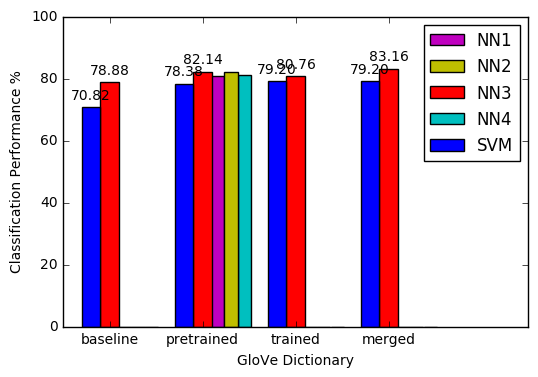
\includegraphics[width=0.8\columnwidth]{glove_NN_SVM.png}
	\caption{Performance of SVM/NN classifiers using GloVe representations obtained by a variety of dictionaries}
	\label{fig:perf1}
\end{figure}

As can be seen from the performance chart, NN outperformed SVM for all cases.
In addition, the best performance is obtained with the largest single layer NN architecture, i.e. NN3, which was the biggest that our resources enabled us.
Second hidden layer, i.e., more nonlinearity never achieved better.
Regarding the GloVe dictionaries, pre-trained vocabulary always lead to better results compared to trained ones, which is expected due to the amount of data used for the pre-trained vocabulary.
However, merging the new words contributes to performance by $1\%$ for both NN an SVM classifiers.
Only interesting thing to notice is the fact that utilization of TFIDF constants as weighting coefficients for GloVe representations does not improve the classification performance.
In fact, we obtained $81.50\%$ classification accuracy with weighted representations of \textit{pretrained} vocabulary and NN3 classifier, whereas the raw representations achieved $82.14\%$.

Furthermore, we investigated the performance of n-grams representation for different window sizes, where it is applied to preprocessed tweets and SVM is utilized as the classifier.
Results are summarized in Figure \ref{fig:perf_ngrams}.

\begin{figure}[h!]
	\centering
	\begin{subfigure}{0.48\columnwidth}
		\centering
		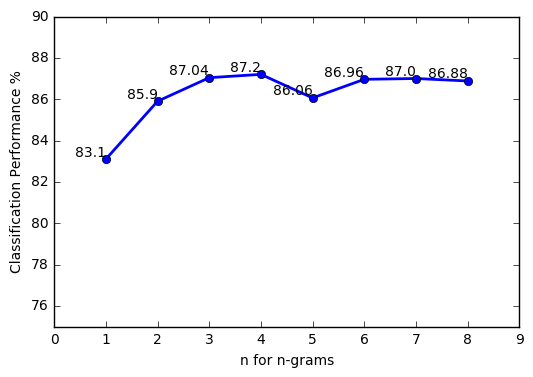
\includegraphics[width=\linewidth]{ngrams.png}
		\caption{n-grams: Performance vs. \textit{n}}
		\label{fig:perf_ngrams}
	\end{subfigure}
	\begin{subfigure}{0.48\columnwidth}
		\centering
		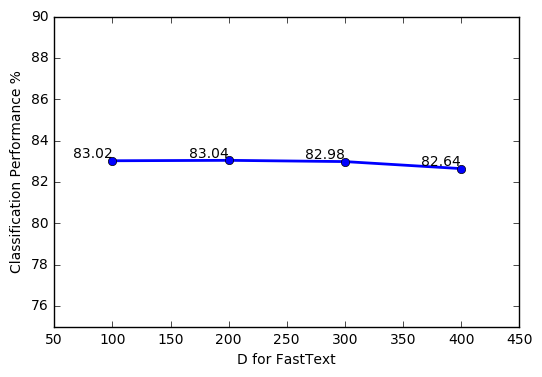
\includegraphics[width=\linewidth]{fasttext.png}
		\caption{FastText: Performance vs. \textit{D}}
		\label{fig:perf_ft}
	\end{subfigure}
\end{figure}


As another test, FastText algorithm is experimented for different dimensions of representations, results of which is given in Figure \ref{fig:perf_ft}.
For all different dimensions, preprocessed dataset is utilized and the classifier is trained with a learning rate $0.05$ by 50 epochs.

In order to further observe the contribution of preprocessing step, we also chose the best-performing n-gram and FastText configurations to apply them to raw data.
results presented in Table \ref{table:preprocess} clearly indicates that proposed preprocessing step adds around $2\%$ to the classification performance.

% Please add the following required packages to your document preamble:
% \usepackage[table,xcdraw]{xcolor}
% If you use beamer only pass "xcolor=table" option, i.e. \documentclass[xcolor=table]{beamer}

\begin{table}[h!]
\centering
\caption{Classification performance ($\%$) with and without preprocessing }
\label{table:preprocess}
\resizebox{\columnwidth}{!}{%
\begin{tabular}{lccc}
\hline
\rowcolor[HTML]{EFEFEF} 
\multicolumn{1}{c}{\cellcolor[HTML]{EFEFEF}\textbf{Algorithm}} & \textbf{w/o preprocessing} & \textbf{w/ preprocessing} & \textbf{Improvement} \\ \hline
\cellcolor[HTML]{EFEFEF}\textbf{4-grams}                       & 85.28                      & 87.20                     & \textbf{1.92}        \\ \hline
\cellcolor[HTML]{EFEFEF}\textbf{FastText, D=200}               & 80.36                      & 83.04                     & \textbf{2.68}        \\ \hline
\end{tabular}
}
\end{table}

The last but not the least, we trained several CNN architectures, where we altered the capacity of the network in order see the limits of the algorithm regarding the training data.
Best performance is achieved when we use a single hidden layer with 128 neurons, where 128 convolutional filters of \{2,3,4,5,6\} neighborhoods are used.
Regarding the computational necessities, instead of cross-validation, we kept randomly chosen 10K samples of training dataset for the validation for all training attempts.
Figure \ref{fig:cnn_train} illustrates the evolution of accuracy during the training.
Roughly speaking, after 18K steps, we suspected model to overfit due to the divergence of accuracy values for training and validation dataset, but as can be seen on the second figure, when we kept training with another randomly chosen validation data due to non-constant seeds, validation performance was better than the training.
The main reason behind this difference is related to the fact that second validation set had been used for the training at the first stage.
Since we didn't have enough time for a training from scratch, we stopped the training at around 30K global steps, which gave us $87.54\%$ test error, which had been $87.48\%$ after 18K global steps.

\begin{figure}[h!]
	\centering
	\begin{subfigure}{0.8\columnwidth}
		\centering
		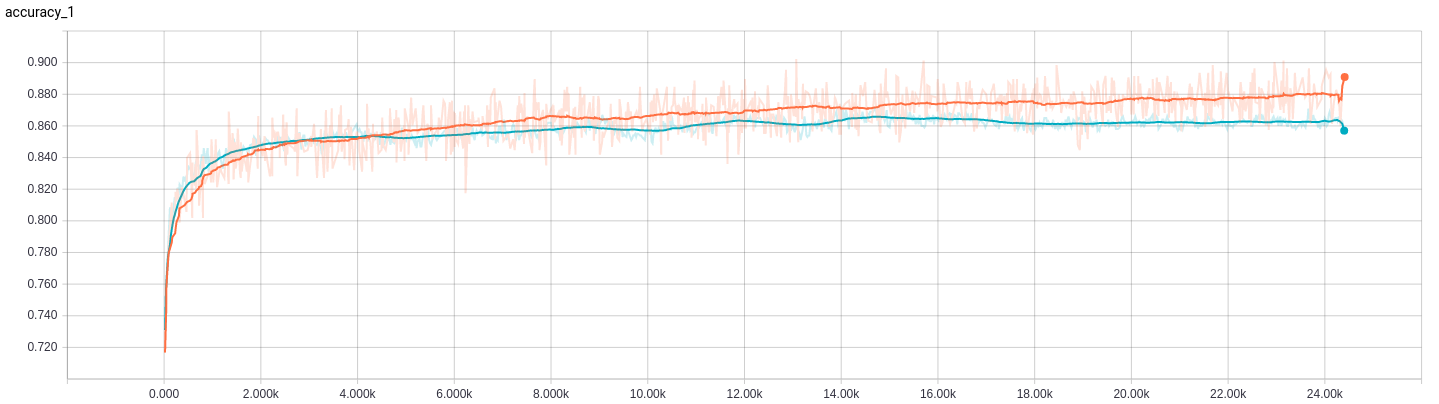
\includegraphics[width=\linewidth]{accuracy1.png}
		\caption{}
		\label{fig:18k}
	\end{subfigure}
	\begin{subfigure}{0.8\columnwidth}
		\centering
		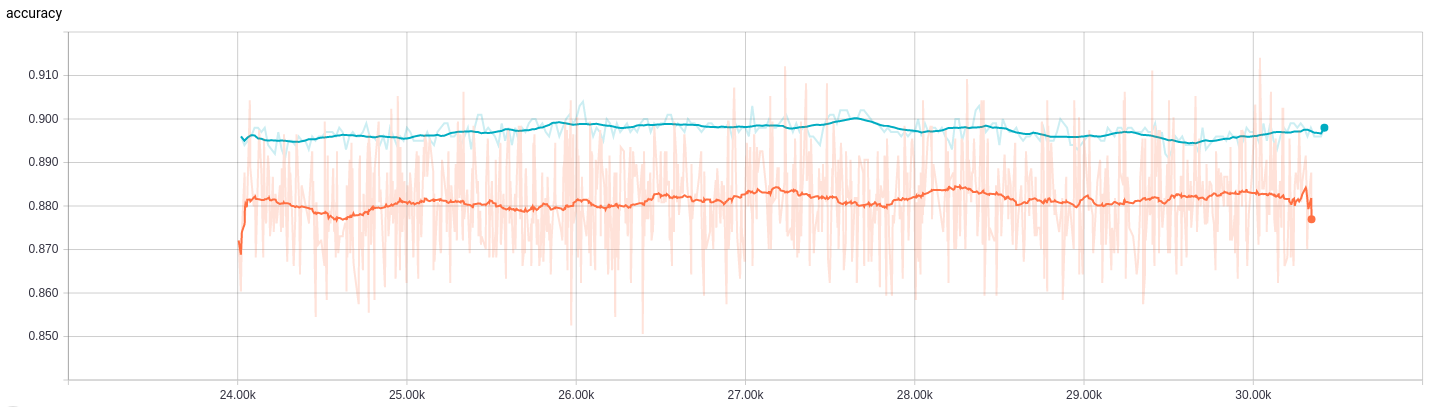
\includegraphics[width=\linewidth]{accuracy2.png}
		\caption{}
		\label{fig:30k}
	\end{subfigure}
	\caption{Evolution of accuracy values for training(orange, smoothed) and validation(blue) datasets for \ref{fig:18k} first 18K steps and \ref{fig:30k} remaining 12K steps}
	\label{fig:cnn_train}
\end{figure}

When we increased or decreased the capacity of networks by increasing/decreasing the number of filters per neighborhood sizes as well as the number neighborhoods, or adding another hidden layer before soft-max classifier, performance always got worse.
If we increased the capacity, decay in the performance is related to overfitting and if we decrease the capacity, deterioration can be due to insufficient representational power.
